\section{Method}

\subsection{Introducing noise}
To ensure model robustness in real-world conditions, we introduced two types of noise to the images: Gaussian noise and Salt and Pepper noise. 
Gaussian noise simulates random intensity variations that might occur due to poor lighting or sensor noise, while Salt and Pepper noise represents random white and black pixels that could appear due to dead pixels or transmission errors.
Additionally, we introduced noise by flipping and rotating images, which simulates diffrent camera angels and orientations.

\begin{figure}[H]
    \centering
    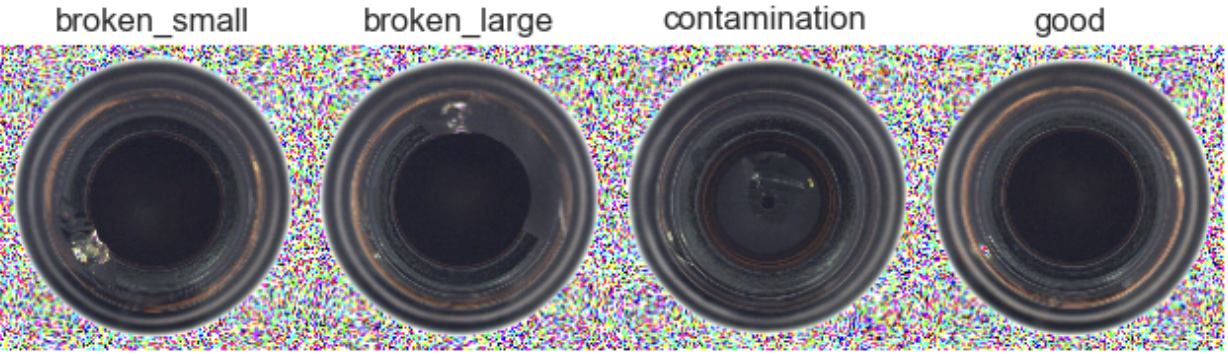
\includegraphics[scale=0.55]{src/images/dataset_w_gnoise.png}
    \caption{Images with Gaussian noise.}
    \label{fig:Gnoise}
\end{figure}
\begin{figure}[H]
    \centering
    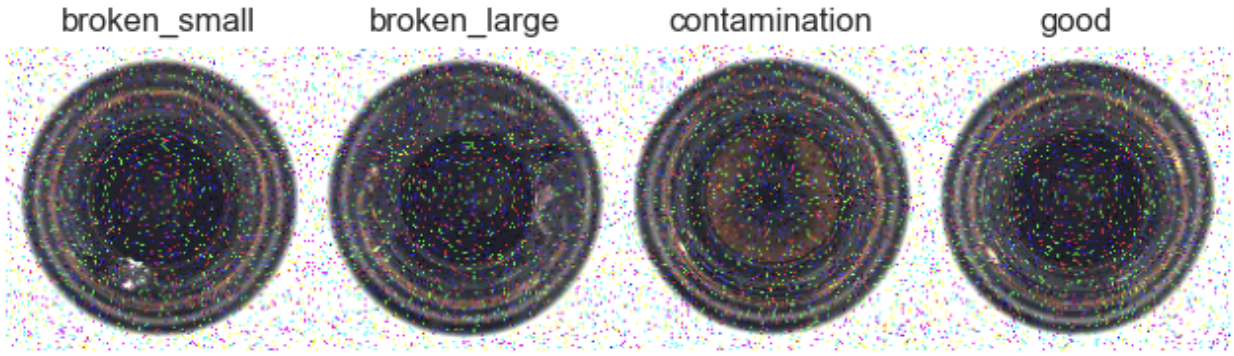
\includegraphics[scale=0.55]{src/images/dataset_w_snp.png}
    \caption{Images with Salt and Pepper noise.}
    \label{fig:snpnoise}
\end{figure}
